\documentclass[12pt]{article}
\usepackage{graphicx}
\usepackage{float}
\usepackage{amsmath}
\usepackage{amssymb}
\begin{document}
\title{Electrical Engineering 113, Homework 4}
\date{May 8th, 2019}
\author{Michael Wu\\UID: 404751542}
\maketitle


\section*{Problem 1}

We can write that \(z[n]=x[n]\circledast x[n]\), which can be easily seen by using a flip and drag method. Since
convolution in the time domain corresponds to multiplication in the frequency domain with a scale of \(N\), we obtain
the following result. Let \(r_k\) be the DTFS coefficients for \(z[n]\) and \(s_k\) be the DTFS coefficients for \(x[n]\).
\[r_k = 3s_k^2\]

\section*{Problem 2}

\paragraph{a)}

We know that the DTFT of \(a^nu[n]\) is \(\frac{1}{1-ae^{-j\Omega}}\). Then we will rewrite the function \(x[n]\) as follows.
\begin{align*}
    x[n] &= \left(\frac{1}{2}\right)^{n-3} u[n] + \left(\frac{1}{3}\right)^n u[n-1]\\
    &=8\left(\frac{1}{2}\right)^n u[n] + \frac{1}{3}\left(\frac{1}{3}\right)^{n-1} u[n-1]
\end{align*}
By substituting in the expression for the DTFT of \(a^nu[n]\) and applying the time shifting property we can obtain the following result.
\[X(\Omega)= \frac{8}{1-\frac{1}{2}e^{-j\Omega}} + \frac{e^{-j\Omega}}{3\left(1-\frac{1}{3}e^{-j\Omega}\right)}\]

\paragraph{b)}

For the cosine term, we begin with the DTFT for \(x[n]=1\) which is shown below.
\[2\pi \sum_{m=-\infty}^\infty \delta(\Omega-2\pi m)\]
We can then apply the modulation property to this to obtain the DTFT for the cosine term.
\[\pi\sum_{m=-\infty}^\infty\left(\delta\left(\Omega-\frac{\pi}{3}-2\pi m\right) + \delta\left(\Omega+\frac{\pi}{3}-2\pi m\right)\right)\]
We will use the DTFT of \(a^nu[n]\) again which gives us the following result.
\[X(\Omega) = \frac{4}{1-\frac{1}{4}e^{-j\Omega}}+\pi\sum_{m=-\infty}^\infty\left(\delta\left(\Omega-\frac{\pi}{3}-2\pi m\right)
+\delta\left(\Omega+\frac{\pi}{3}-2\pi m\right)\right)\]

\section*{Problem 3}

\paragraph{a)}

Begin by finding the IDTFT of \(\text{rect}\left(\frac{\Omega}{\frac{\pi}{6}}\right)\).
\begin{align*}
    x[n] &= \frac{1}{2\pi}\int_{-\pi}^\pi \text{rect}\left(\frac{\Omega}{\frac{\pi}{6}}\right) e^{j\Omega n}\,d\Omega\\
    &=\frac{1}{2\pi}\int_{-\frac{\pi}{6}}^\frac{\pi}{6} e^{j\Omega n}\,d\Omega\\
    &=\frac{1}{2\pi jn}\left.e^{j\Omega n}\right|_{-\frac{\pi}{6}}^\frac{\pi}{6}\\
    &=\frac{1}{2\pi jn}(e^{j\frac{\pi}{6} n}-e^{j\frac{\pi}{6} n})\\
    &=\frac{\sin(\frac{\pi}{6} n)}{\pi n}
\end{align*}
Then we can apply time shifting and scale by a constant to obtain the following result.
\[x[n] = \frac{\sin(\frac{\pi}{6} (n-2))}{2(n-2)}\]

\paragraph{b)}

From Parseval's Theorem we have the following relationship.
\[\sum_{n=-\infty}^\infty |x[n]|^2 = \frac{1}{2\pi}\int_{-\pi}^{\pi} \left|\frac{\pi}{2}\text{rect}\left(\frac{\Omega}{\frac{\pi}{6}}\right) e^{-j2\Omega}\right|^2\,d\Omega\]
We then obtain the following result.
\[\frac{\pi}{8}\int_{-\frac{\pi}{6}}^\frac{\pi}{6} d\Omega = \frac{\pi^2}{24}\]

\section*{Problem 4}

\paragraph{a)}

Take the case where \(n\neq 0\).
\begin{align*}
    x[n] &= \frac{1}{2\pi}\int_{-\pi}^\pi X(\Omega) e^{j\Omega n}\,d\Omega\\
    &=\frac{1}{2\pi}\int_{-\omega_c}^{\omega_c} e^{j\Omega n}\,d\Omega\\
    &=\frac{1}{2\pi jn}\left.e^{j\Omega n}\right|_{-\omega_c}^{\omega_c}\\
    &=\frac{1}{2\pi jn}(e^{j\omega_c n}-e^{j\omega_c n})\\
    &=\frac{\sin(\omega_c n)}{\pi n}
\end{align*}
Take the case where \(n=0\).
\begin{align*}
    x[n] &= \frac{1}{2\pi}\int_{-\pi}^\pi X(\Omega) e^{j\Omega n}\,d\Omega\\
    &=\frac{1}{2\pi}\int_{-\omega_c}^{\omega_c}\,d\Omega\\
    &=\frac{\omega_c}{\pi}
\end{align*}
Thus we have the following result.
\[x[n]=\begin{cases}\frac{\omega_c}{\pi}&n=0\\ \frac{\sin(\omega_c n)}{\pi n}& n\neq 0\end{cases}\]

\paragraph{b)}

\begin{align*}
    \tilde{X}(\Omega) &= \sum_{n=-\infty}^\infty x[n] e^{-j\Omega n}\\
    &= \frac{\omega_c}{\pi} + \sum_{n=-\infty, n\neq 0}^\infty \frac{\sin(\omega_c n)}{\pi n} e^{-j\Omega n}
\end{align*}

\paragraph{c)}

The plots are shown below.
\begin{figure}[H]
    \begin{center}
        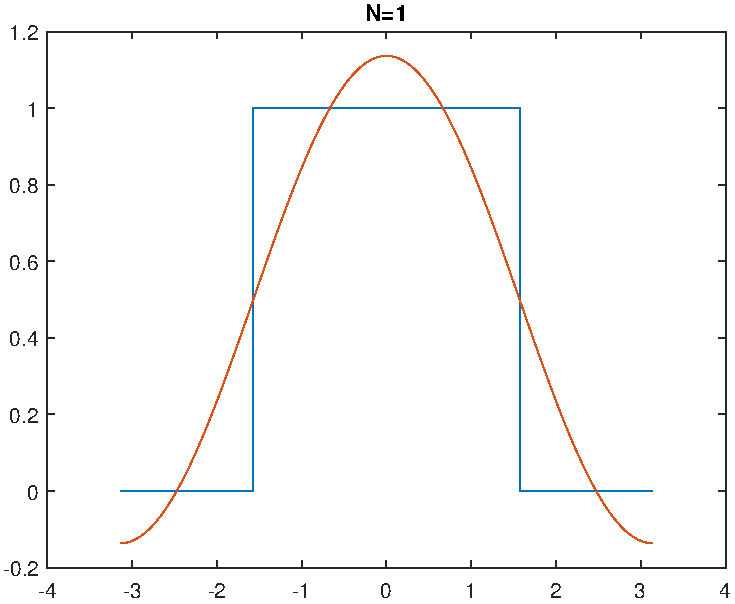
\includegraphics[width=1.5in]{problem4c-1.pdf}
        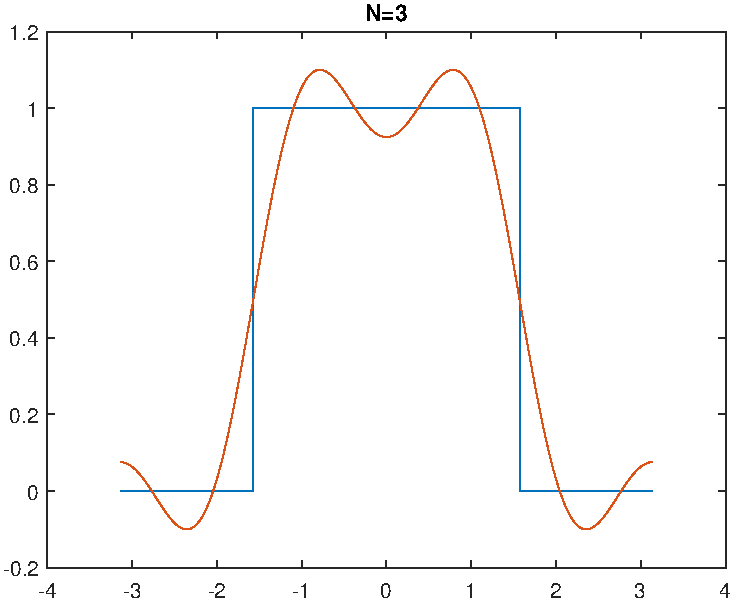
\includegraphics[width=1.5in]{problem4c-3.pdf}
        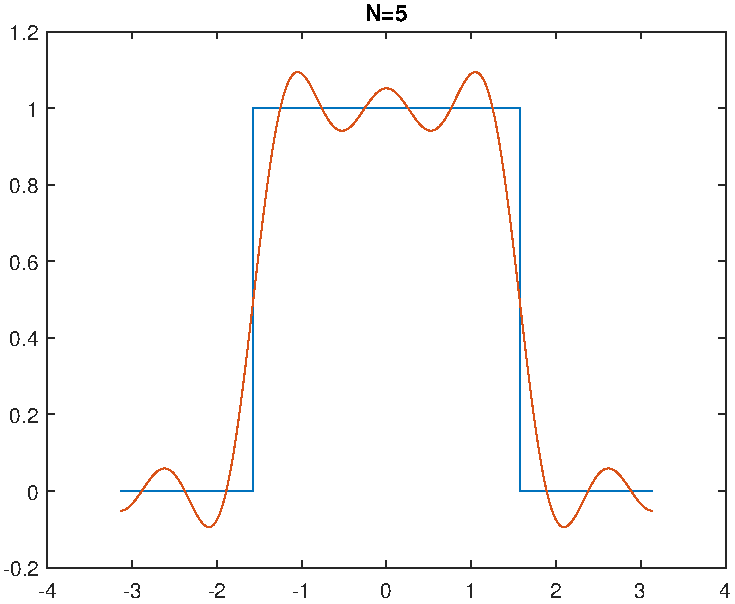
\includegraphics[width=1.5in]{problem4c-5.pdf}
        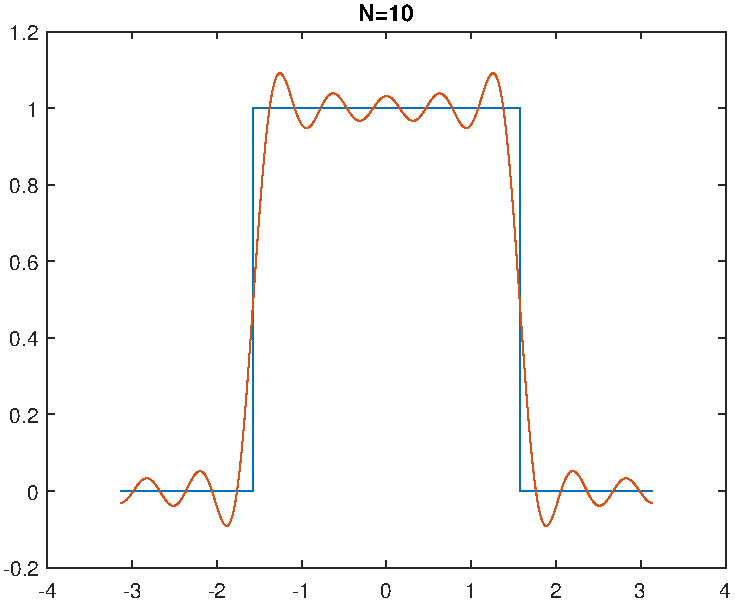
\includegraphics[width=1.5in]{problem4c-10.pdf}
        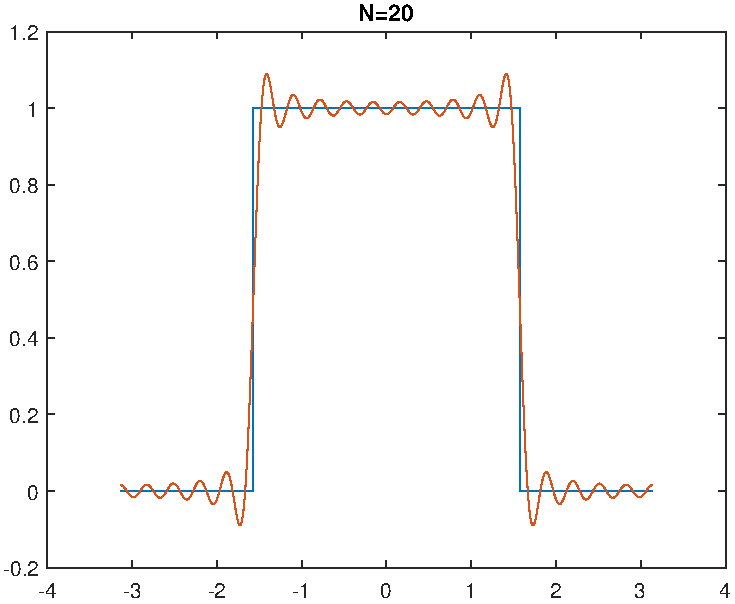
\includegraphics[width=1.5in]{problem4c-20.pdf}
        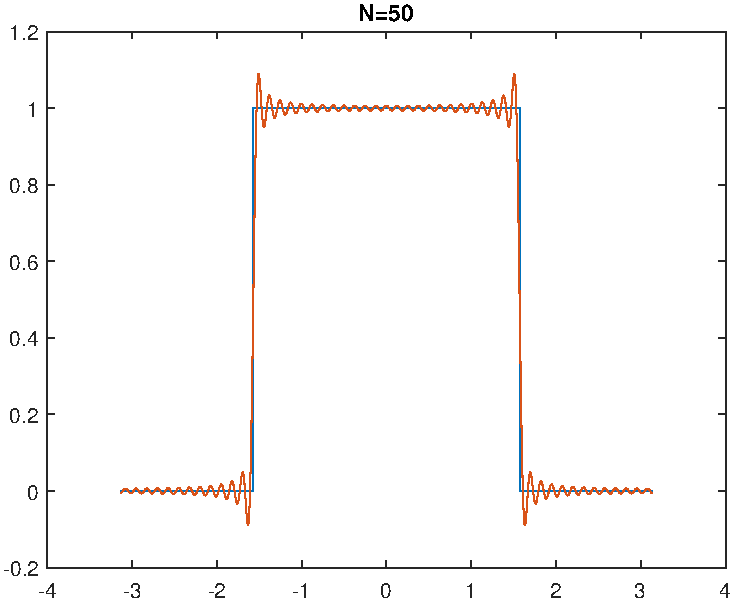
\includegraphics[width=1.5in]{problem4c-50.pdf}
    \end{center}
\end{figure}

\paragraph{d)}

The plots of \(\tilde{X}(\Omega)\) begin to more closely resemble \(X(\Omega)\) as \(N\) increases, but there is
some overshoot at the discontinuities in \(X(\Omega)\). This is the Gibbs phenomenon.

\section*{Problem 5}

\paragraph{a)}

I ran the following script.
\begin{verbatim}
A=double(imread('Lena.bmp'));
[U, S, V]=svd(A);
singvals=diag(S);
indices=find(singvals >= 0.01 * max(singvals));
U_red=U(:, indices);
S_red=S(indices, indices);
V_red=V(:, indices);
A_red=U_red * S_red * V_red';
imshow(uint8(A_red));
export_fig problem5a.pdf
\end{verbatim}
This produced the following output.
\begin{figure}[H]
    \begin{center}
        
\includegraphics[width=3in]{problem5a.pdf}
    \end{center}
\end{figure}

\paragraph{b)}

We need \(53\times 512 + 53^2 + 53\times 512 = 57081\) real values to store this image. This is \(21.775\%\) the size
of the size of the original image \(A\).

\end{document}